\chapter{Introduction}

\section{Motivation and Background}

Leakage in water distribution systems is a major global problem with economic, environmental, and operational consequences. Estimates from the World Bank show that developing countries lose tens of millions of cubic meters of treated water each day due to pipe leakage. This volume could otherwise supply a large population \cite{kingdom2006}.\\

\begin{figure}[h!]
    \centering
    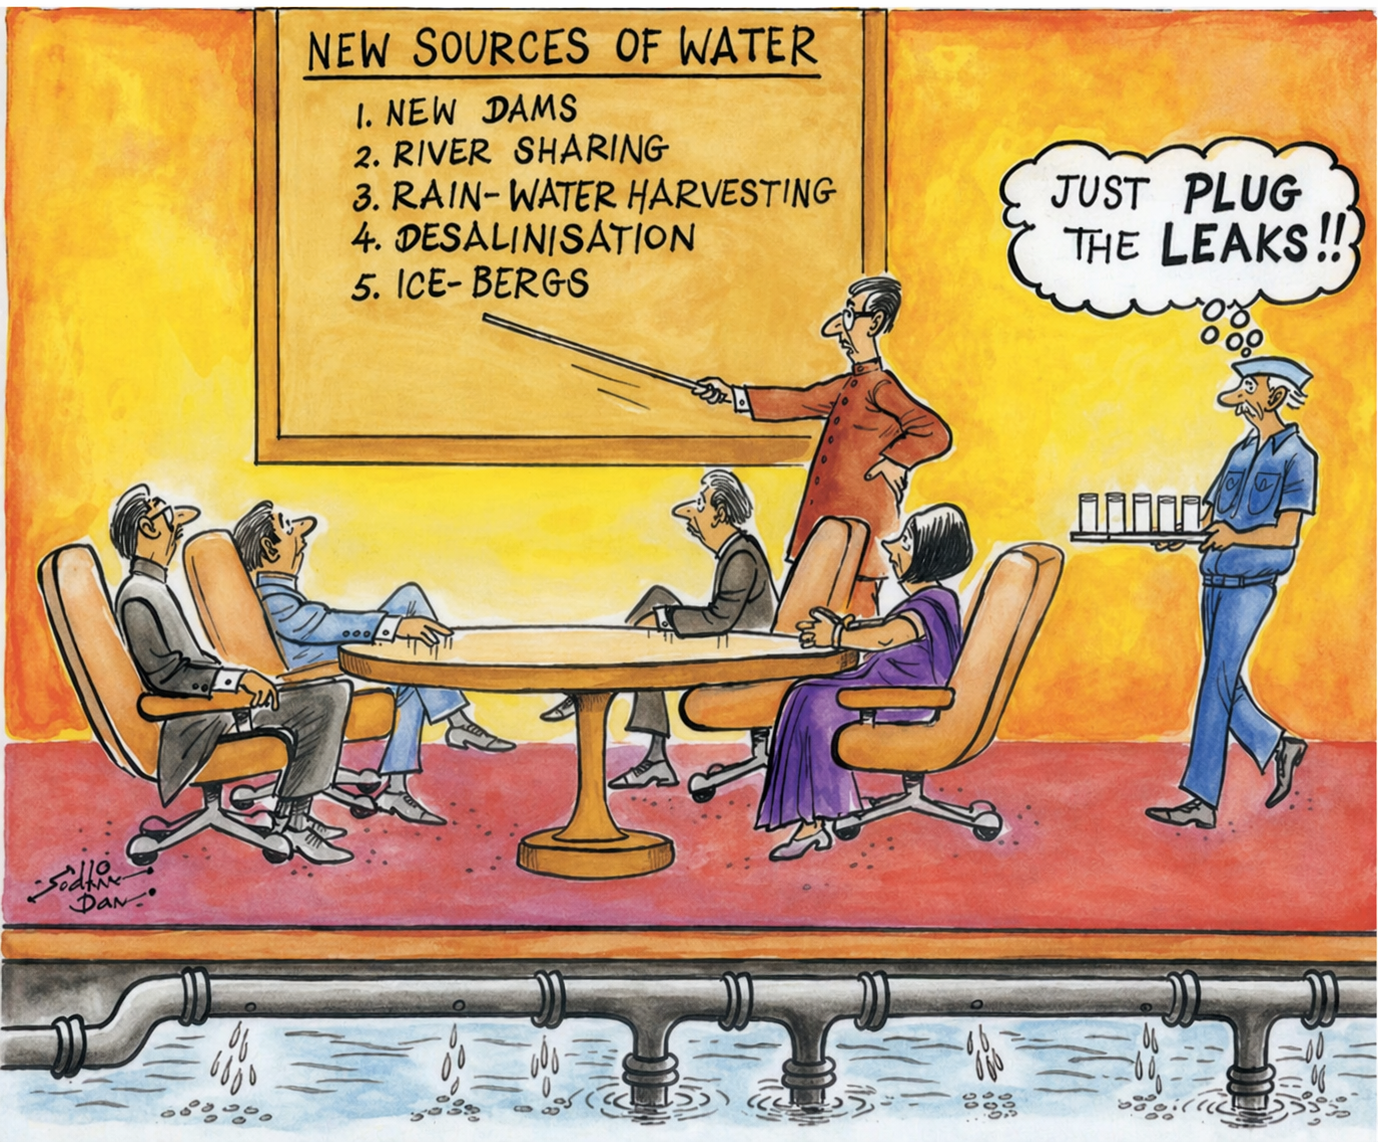
\includegraphics[width=0.6\linewidth]{images/plug_the_leaks.png}
    \caption{Illustration from the Water and Sanitation Program of the World Bank \cite{iwa2007} (Quality enhanced by ChatGPT) }
    \label{fig:plug_the_leaks}
\end{figure}

These losses are often described as non-revenue water (NRW), which refers to the difference between the volume of water entering the distribution system and the volume billed to consumers. NRW includes physical losses caused by leakage as well as other forms of water that do not generate revenue. Recent global estimates indicate that NRW amounts to approximately 346 million $m^3$/day, or 126 billion $m^3$/year, which equates to 30\% of all distributed water worldwide, with an annual cost of around USD 39 billion \cite{liemberger2018}. Pipe leaks may also damage surrounding infrastructure and pose environmental and public health risks \cite{qi2018}. Leaks may reverse the flow direction, potentially causing water quality issues, and significantly increase flow velocities, which can dislodge biofilms and further deteriorate water quality. \\

Leakage levels vary significantly between countries. In Norway, water distribution systems experience some of the highest leakage rates in Europe. The average water loss is around 30\%, and in several systems, more than 40\% of treated drinking water is lost due to leakage in the network \cite{norskvann2026}.\\

Leak detection and repair are often difficult and expensive in practice. Many leaks occur underground and may remain undetected for long periods, especially when water does not reach the surface. Once a leak is suspected, utilities often rely on field inspections, acoustic surveys, and other local investigations to estimate its location before excavation begins \cite{hu2021}. This process requires significant time and cost because excavation is disruptive, and the exact leak location often remains uncertain until digging begins. This limitation has increased interest in software-based and data-driven detection and localization methods.\\

Specifically, there is a practical interest in identification methods that rely only on head and flow measurements. These variables are commonly measured in real pipeline systems, which makes them suitable for practical monitoring applications \cite{hu2021}. Available sensors do not always sample at a sufficiently high frequency to detect hydraulic transients, which may occur over very short time scales. In such cases, steady-state information provides a more reliable basis for analysis. This makes methods based on steady-state inlet and outlet measurements of head and flow relevant to investigate.\\

The detection and localization of multiple simultaneous leaks has received limited attention in the literature. It is pointed out in \cite{torres2024} that truly simultaneous leak events are generally considered unlikely. Despite this, the problem remains relevant in practice. In older water networks that have not been continuously monitored, multiple defects may already be present by the time sensors are installed, and measurements are collected. Based on the available hydraulic data, this situation is equivalent to observing multiple concurrent leaks. This provides clear motivation to investigate whether several leaks can be identified in pipe segments between available measurement points.

\newpage
\section{Master's Thesis Assignment}

This section outlines the master's thesis assignment. It begins with a description of the task, followed by the delimitations that set the scope of the work. Finally, there is a brief discussion of the work's relevance to sustainability.

\subsection{Task Description} \label{sec:task_desc}

Consider a pipe of length \gls{ell}, where \gls{z} $\in [0, \ell]$ denotes position along the pipe. Assume steady-state operation, and let
\[
q : [0,\ell] \to \mathbb{R}_{\geq0}, \qquad h : [0,\ell] \to \mathbb{R}_{\geq0}
\]
denote the volumetric discharge and piezometric head (from now regarded as flow and head for brevity). Thus, \gls{qz} and \gls{hz} represent the flow and head at position \gls{z}, which are both assumed strictly positive along the pipe. Suppose \gls{n} leaks occur at locations
\[
0 < z_1 < \dots < z_n < \ell,
\]
with corresponding leak discharges $\tilde q_1,\dots,\tilde q_n$, where \gls{tildeqi} and \gls{zi} correspond to the $i$-th leak. Assuming small leak openings, each leak is modeled as a valve by
\[
\tilde{q}_i = c_i \sqrt{h(z_i)},
\]
where \gls{ci} $>0$ is a constant discharge coefficient characterizing the $i$-th leak. 
The steady-state head loss along the pipe is governed by
\begin{equation}
\label{eq:task_desc_ufunc}
\frac{dh}{dz} = -U(q(z)),
\end{equation}
where \gls{U} $:[0,\infty)\to[0,\infty)$ is smooth and strictly increasing. For notation purposes, let the flow and head at the inlet and outlet be defined by
\[
\text{\gls{q0}} := q(0), \qquad \text{\gls{ql}} := q(\ell), \qquad
\text{\gls{h0}} := h(0), \qquad \text{\gls{hl}} := h(\ell).
\]
Since flow is conserved between leak locations, $q$ is piecewise constant. Introducing $z_0:=0$ and $z_{n+1}:=\ell$, the flow is given by
\[
q(z)=\text{\gls{qi}}:=
\begin{cases}
q_0, & \text{for } z \in [0, z_1), \quad i = 0, \\[6pt]
q_0 - \sum_{k=1}^{i} \tilde{q}_k, & \text{for } z \in [z_i, z_{i+1}), \quad i = 1, \dots, n,
\end{cases}
\]
where also $q_n=q_{\ell}$ for notation consistency. From \cref{eq:task_desc_ufunc}, it follows that the head is continuous and piecewise linear along the pipe. Let
\[
L_{i+1} := z_{i+1}-z_{i},
\qquad i=0,\dots,n,
\]
denote the lengths of the non-leaking segments, so that
\[
\sum_{i=1}^{n+1} \text{\gls{Li}} = \ell.
\]
The head at the $i$-th leak location is denoted by
\[
\text{\gls{hi}} := h(z_i), \qquad i=1,\dots,n,
\]
and for notation consistency, let $h_{n+1}:=h_{\ell}$. The notation for a pipe is illustrated in \autoref{fig:leak_notation}.\\

\begin{figure}[h!]
    \centering
    \input{figures/tikz_pipe}
    \caption{Notation used for a pipe with $n$ leaks.}
    \label{fig:leak_notation}
\end{figure}

Suppose the flow and head at the pipe's inlet and outlet can be measured at \gls{m} different steady-state operating points. For the $j$-th operating point, let
\[
\text{\gls{y0}} :=\begin{bmatrix}
    h_0^{(j)} \\[0.4em]
    q_0^{(j)}
\end{bmatrix}, \quad
\text{\gls{yl}} := \begin{bmatrix}
    h_{\ell}^{(j)} \\[0.4em]
    q_{\ell}^{(j)}
\end{bmatrix}, \quad
j=1,\dots,m,
\]
define the vectors of inlet and outlet measurements. The complete matrices of inlet and outlet measurements are defined by
\[
\text{\gls{M0}}
:=
\begin{bmatrix}
y_0^{(1)} & \cdots & y_0^{(m)}
\end{bmatrix} \in\mathbb{R}^{2\times m},
\qquad
\text{\gls{Ml}}
:=
\begin{bmatrix}
y_{\ell}^{(1)} & \cdots & y_{\ell}^{(m)}
\end{bmatrix} \in\mathbb{R}^{2\times m}.
\]
For notation purposes, let all measurements be defined by
\[
\text{\gls{M}}
:=
\begin{bmatrix}
\mathcal{M}_0 \\[0.4em] 
\mathcal{M}_{\ell}
\end{bmatrix} \in\mathbb{R}^{4\times m} 
\]
and \gls{y} $:=\begin{bmatrix}
    \text{\gls{y0}} \\[0.4em]
    \text{\gls{yl}}
\end{bmatrix} \in \mathbb{R}^4$ is defined as the $j$-th column of \gls{M}.\\

\begin{definition}{Leak Identification Problem}{leak-identification}
For some leak parameters $\vartheta := \begin{bmatrix}
    z_1 & \cdots & z_n & c_1 & \cdots & c_n
\end{bmatrix}^\top$, assume there exists a function
\[
\mathcal{F}_{\mathcal{M}_0}(\vartheta) = \mathcal{M}_\ell,
\]
parametrized by some fixed inlet measurements \gls{M0}, which produces the outlet measurements \gls{Ml}. The leak identification problem is the inverse problem of recovering leak parameters $\vartheta$ from \gls{M0} and \gls{Ml}:
\[
\vartheta = \mathcal{F}_{\mathcal{M}_0}^{\,-1}(\mathcal{M}_\ell)
\]
\end{definition}

\begin{definition}{Leak Identification Problem (alt)}{leak-identification2}
Let the input-output relation of a pipe with $n$ leaks be defined by
\begin{equation*}
    \mathcal{P}_n(\vartheta) : \mathcal{M}_0 \mapsto \mathcal{M}_\ell,
\end{equation*}
where $\vartheta := \begin{bmatrix}
    z_1 & \cdots & z_n & c_1 & \cdots & c_n
\end{bmatrix}^\top$ denotes the leak parameters.\\

The leak identification problem is to identify a parameter vector $\vartheta$ that is consistent with the observed input-output behavior
given by $\mathcal{M}_0$ and $\mathcal{M}_\ell$.
\end{definition}

\begin{samepage}
The following tasks should be performed:
\begin{enumerate}
    \item Literature review (see \cite{peralta2023}, \cite{molno2024parallel}, \cite{molno2024conditions} for a starting point). \\

    \item Assuming that the function \gls{U}, the number of leaks \gls{n}, and the pipe length \gls{ell} are known, develop and implement a method for solving the leak identification problem as defined in \autoref{def:leak-identification}.\\

    % \item Assuming that the function \gls{U}, the number of leaks \gls{n}, and the pipe length \gls{ell} are known, develop and implement a method for identifying the leak locations $(z_1,\dots,z_n)$ and the corresponding discharge coefficients $(c_1,\dots,c_n)$ from the measurement collection \gls{M}, consisting solely of inlet and outlet measurements obtained from \gls{m} different steady-state operating points.\\

    \item Investigate the maximum number of leaks feasible to identify.\\
    
    \item Perform simulated tests to investigate the performance of the method in the idealized setup (\gls{U}, \gls{n}, and \gls{ell} are known).\\

    \item Investigate how the method performs when parameters are uncertain, or noise is introduced to measurements.\\
\end{enumerate}
\end{samepage}

\newpage
\subsection{Delimitations}

The following delimitations restrict the scope of the work:

\begin{itemize}

\item \textbf{Leak detection:}
The problem of detecting leaks is not addressed. Under the adopted assumptions, the presence of a leak is trivial, since a discrepancy between the inlet and outlet flow indicates leakage. References such as \cite{isermann1997} and \cite{blanke2006} describe detection methods and alarm systems in detail.\\

\item \textbf{Number of leaks:}
The case of a single leak ($n = 1$) is not considered, since this problem is well defined and can be solved analytically. It is treated as trivial in this context. The thesis focuses on multiple simultaneous leaks ($n \geq 2$).\\

\item \textbf{System scope:}
The system consists of a single pipeline segment. Pipe networks with branches or junctions are not considered.\\

\item \textbf{Model assumptions:}
To simplify the derivations, the hydraulic resistance function will be limited to the quadratic form (based on the derivation in \autoref{chap:model})
\[ U(q(z)) = \theta q^2(z), \]
where \gls{theta} is assumed to be a known and constant friction parameter. It should be noted that these assumptions are not required by the method, and more advanced friction models, or parameters as functions of $z$, could be incorporated.\\

Leaks are assumed to be small relative to the total flow. This ensures that flow and head are non-zero at the outlet. The flow is assumed unidirectional along the pipe, with leaks limited only to outward flow and no external inflow.\\

Only steady-state conditions are considered. Transient effects such as pressure waves and time-dependent flow dynamics are excluded.\\

The main analysis follows idealized conditions, without modeling or measurement errors, and assumes the number of leaks is known. The aim is to isolate the problem's fundamental theoretical properties and limitations. This provides insight into the underlying challenges that remain relevant under non-ideal assumptions, since the limitations present in the ideal case also constrain more realistic and complex scenarios.\\

For completeness, a brief extension in \autoref{sec:n_not_known} considers the case where the number of leaks is unknown, and \autoref{sec:mod_err} examines the impact of model and measurement errors. For space reasons, only modeling errors in \gls{theta} are considered, since it is assumed to be the most difficult parameter to estimate in practice.\\

\item \textbf{Measurements:}
In a practical situation, \gls{M} would come from measuring a physical system operating at different steady-states. Due to data availability and the scope of the problem, $\mathcal{M}$ will be generated in this work through simulation, where the pipe parameters \gls{ell} and \gls{theta} are known exactly. The measurements are therefore free of both model error and measurement noise.\\

\end{itemize}

\subsection{Sustainability Relevance}

This work relates to sustainability by reducing water losses and improving resource efficiency in water distribution systems. Lower leakage rates reduce unnecessary water extraction and the energy required for treatment and pumping, thereby decreasing the overall environmental footprint of water supply operations.\\

These aspects are linked to several of the United Nations Sustainable Development Goals \cite{un_goals}. In particular, the work supports SDG 6 (Clean Water and Sanitation) by improving water-use efficiency and SDG 9 (Industry, Innovation and Infrastructure) by developing enhanced monitoring and diagnostic methods. It also contributes to SDG 12 (Responsible Consumption and Production) by promoting more efficient resource use and reducing waste.

\section{Overall Organization of Work}

The project combined method development, numerical testing, and mathematical analysis of the underlying problem structure. The work was primarily theoretical, with additional focus on practical implementation and applicability to real-world problems. The main objective was to develop a program capable of solving the leak identification problem defined in \autoref{def:leak-identification}. The developed framework was evaluated using simulated data, where performance was assessed through empirical results.\\

The work presented in this thesis was initiated independently for the project and was not based on existing implementations, previously collected datasets, or prior development work. The initial stages of the project, therefore, focused on establishing the theoretical framework and developing the associated software tools from first principles.\\

An extensive literature review was conducted before and during the development process. Alongside traditional academic search engines, the large language model, ChatGPT \cite{chatgpt}, supported the literature search process. Detailed descriptions of research topics and information needs were provided to the model to identify potentially relevant publications. This approach made it possible to find relevant work and conceptual connections even when suitable terminology was unknown or difficult to express through standard keyword searches. Previous studies have shown that such models can support literature search and screening tasks within scientific domains \cite{jin2024pubmedandbeyond}, \cite{dennstadt2024titleandabstract}, \cite{delgado-chaves2025transforming}. The identified papers were then studied in detail, and their references were used to further expand the review. Google Scholar and arXiv were used to access specific publications, while Connected Papers \cite{connectedpapers} was used to improve the coverage of related work within the field.\\

To support the software development process, AI-assisted programming tools such as Codex \cite{codex} and Cursor \cite{cursor} were used for rapid prototyping and agent-based debugging. These tools enabled efficient testing of ideas and accelerated the development process. For numerical simulations, NTNU provided access to dedicated computing resources, enabling computationally demanding workloads to be executed in parallel. The total simulation time is estimated to be approximately 200 hours.\\

Throughout the writing process, ChatGPT was used to reformulate draft text, format mathematical expressions, and assist with implementing TikZ figures. Grammarly \cite{grammarly} has been used throughout the writing of this report for spell checking, improving sentence structure, and rewording. Additional details regarding the use of AI tools are provided in the attached AI declaration.

\newpage
\section{Structure of the Report}

\renewcommand{\descriptionlabel}[1]{\normalfont #1}
\begin{description}[itemsep=2pt, topsep=0pt, parsep=0pt]
    \item[Chapter 1] presents the motivation for the work, defines the assignment, and describes the organization of the project.

    \item[Chapter 2] gives an overview of the studied literature and an analysis of relevant published methods.

    \item[Chapter 3] introduces the theoretical background for nonlinear residual problems and optimization methods, providing the essential knowledge needed to follow the methods and algorithms developed.

    \item[Chapter 4] derives the mathematical model for a water pipe with leaks used in this work.

    \item[Chapter 5] presents how the problem is formulated as a nonlinear residual problem and proposes a solver design to find a solution. 

    \item[Chapter 6] performs a mathematical analysis of the residual function to investigate two things. First is how the measurements affect the solution space, and how different steady-state operating points can be chosen to improve the identifiability of the leaks. Secondly, how the increase in the number of leaks affects the feasibility of identifying them. 

    \item[Chapter 7] compares the proposed method against a published method and further tests it using an extensive test framework, yielding empirical results on the method's performance. The chapter also presents how the method performs when the number of leaks is unknown and when it is introduced to model and measurement errors.

    \item[Chapter 8] discusses the method's limitations based on the results, how the method can be useful in practice, and future work. 

    \item[Chapter 9] concludes the report by summarizing the contributions and achievements.
\end{description}

